\chapter{Versat API 2.0}
\label{chapter:API}

The Versat API, developed in a previous thesis~\cite{valter:deepversat}, has the ability to conceal
the calls to the hardware to avoid changing the program when the hardware changes. 

In this chapter, the new functions that are part of the Versat API will be discussed. The goal
is to make development for Versat just like writing normal code and to be easy to port code the same way
CUDA has done the same to run SIMD code on Nvidia GPUs.

\lstinputlisting[label=listing:versathpp,language=C++,frame=single,breaklines=true,firstline=17,lastline=40,caption=Sample Versat API implementation for the Hardware for Mem functional unit]{./Code/Versat.hpp}

\section{API Architecture}

In figure \ref{newAPI}, a graphic representation of the new API is presented. It has four apparent layers (5 if you count the hardware):

\begin{enumerate}
	\item Complex Mathematical API that is automatically optimized for the Versat Setup you chose. No dev work required
	\item Read/Write using VI and VO for simpler setup of the data. Also includes easier FU functions to set up workloads.
	\item Read/Write configurations for inside Versat Data (Int) or DDR to/from VI/VO (Ext).
	\item Versat API 1.0 where each configuration variable needs to be set up individually
	\item No API. Hardware registers where the values are used inside Versat. 
  \end{enumerate}


\begin{figure}[!htbp]
    \centering
    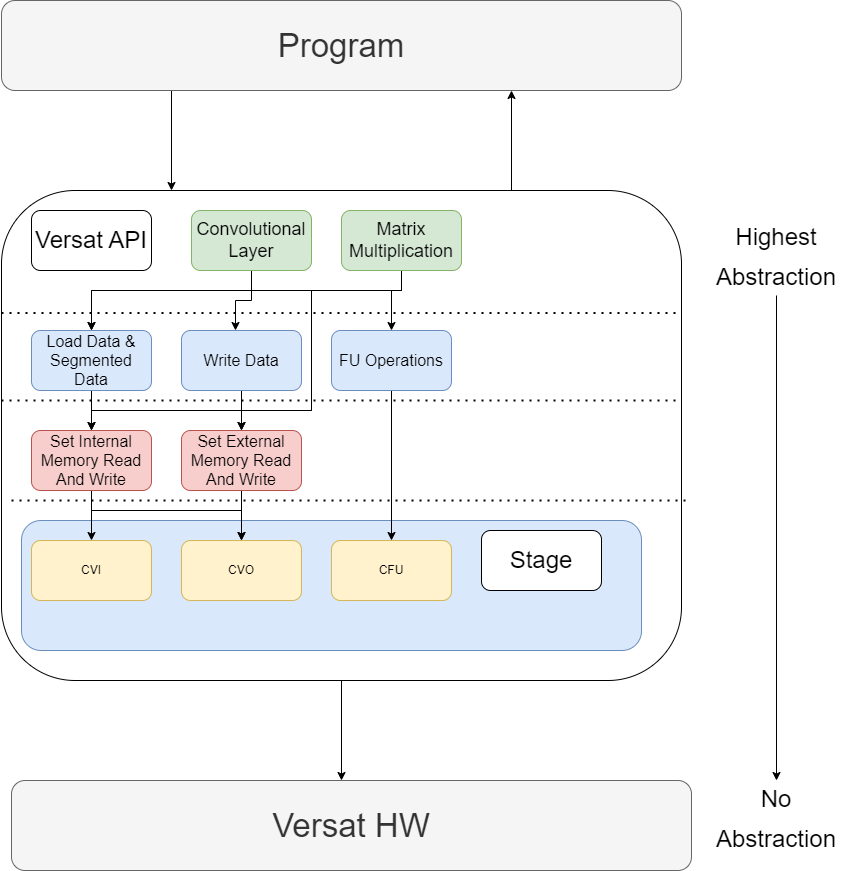
\includegraphics[width=0.7\textwidth]{Figures/VersatMemory.drawio.png}
    \caption{Graphic representation of the new Versat API and its connections}
    \label{newAPI}
\end{figure} 


\section{Memory Operations API}

When utilizing the VI instead of a MEM, the data transfer happens between the functional unit and direct memory access while
on the mem, the CPU writes directly to Versat, wasting CPU cycles. For the API, this means going from a read method that is straightforward
to more configuration methods to set up the read operation from DDR The same happens to Write operations. To address this, seven functions were created in two levels of abstraction:
load\_data(),load\_segmented\_data(),write\_data() that use a lower level functions: set\_IntMem\_Write(),set\_ExtMem\_Write(),set\_IntMem\_Read() and set\_ExtMem\_Read().
The function of the higher abstraction memory functions is to abstract the parameters of the AGU. In the following listing, we have one of the implementations
as an example.

\lstinputlisting[label=listing:loadsegdata,language=C++,frame=single,breaklines=true,firstline=366,lastline=376,caption=Load Segmented Data code]{./Code/versat_configurations.cpp}


Although this means having to write code with the AGUs in mind
and how they function. To avoid it, a new class was created, shown in listing \ref*{listing:accumulator},
to also abstract how the AGU counts loops and approximate 
the code to simple C++ code that runs on a CPU.

\lstinputlisting[label=listing:accumulator,language=C++,frame=single,breaklines=true,firstline=72,lastline=110,caption=Accumulator Class code]{./Code/versatnew.hpp}

To transform from AGU parameters to for loop, it depends on the number of loops pretended to be done. VI AGU is three  cascade Accumulators
and as such, the increment on the second and third accumulators needs to be adjusted, just as shown below.

\lstinputlisting[label=listing:intmemread,language=C++,frame=single,breaklines=true,firstline=77,lastline=86,caption=AGU parameters to Simple forloop parameters transform]{./Code/versat_configurations.cpp}

\section{Matrix Multiplication and Dot Product}

As part of the new API, a matrix multiplication function was added. In listing \ref{listing:matrixmult} the code is presented. First, two Accumulator class variables are initialized.
Afterward, using the two arrays address in DDR, the AGU configurations of the VIs to read from the main memory are set, then the AGU configurations of VI for the data handling inside the Data Engine.
Finally, the function that will write the configuration of a MAC and the store AGU configurations. This last step is optional as the result of this matrix multiplication can be used in the same run
to make other operations e.g.: adding a bias using one of the ALUs to the results.

\lstinputlisting[label=listing:matrixmult,language=C++,frame=single,breaklines=true,firstline=167,lastline=215,caption=Matrix Multiplication Configurations]{./Code/versat_configurations.cpp}

The Dot product function is very similar, the configurations are identical for the data transfer from the main memory to the VIs. In the inside loops of the VIs, instead of three  loops, we only need to use 
1.

\section{Generic Convolution}

As explained in chapter \ref*{chapter:Background}, convolutional neural networks are a type of neural nets that are 
used mostly in image and object recognition by using convolutional layers. To run a convolutional layer on Versat with
optimized performance, the configurations must be written with regard to several parameters:

\begin{enumerate}
	\item Memory Sizes used in VI and VO. The amount of data that can be stored at once. It determines the number of outputs done per run.
	\item Functional Units used in the Data Engine. Here it's about the lowest common denominator, i.e. the bottleneck in the Data Engine determines the number of outputs done simultaneously.
  \end{enumerate}
 
This function has a total of 20 variables calculated at the start before the Versat configurations are written. The most important
variables are the following:

\begin{itemize}
	\item output height (h) and width (w) of the resulting matrix from the convolution.
	\item Number of outputs done simultaneously, also known as pipeline width (nOutputs). This value is pre-compiled as it depends on only Versat Configurations.
	\item Number of outputs that can be done per VI (y) in a single run and its variations. Outputs total (y\textsubscript{2}), Output Lines per VI (y\textsubscript{3}) Output Lines total (y\textsubscript{4}).
The value of y4 and y2 decide the different configuration scenarios.
	\item Resource Allocation Variables
which are explained in subsection \ref*{ConvolutionScenarios}
	\item Address Variables
	\item AGU Configuration Variables
  \end{itemize}

The hard part of the algorithm is to allocate the data in the most efficient way possible and to create the AGU configurations
for the VIs and VOs. For this algorithm, the CGRA will act like a GPU pipeline where several "threads" will exist
that will output one point every k\textsuperscript{2} cycles, where k is the kernel size used in the convolution.

\begin{figure}[!htbp]
    \centering
    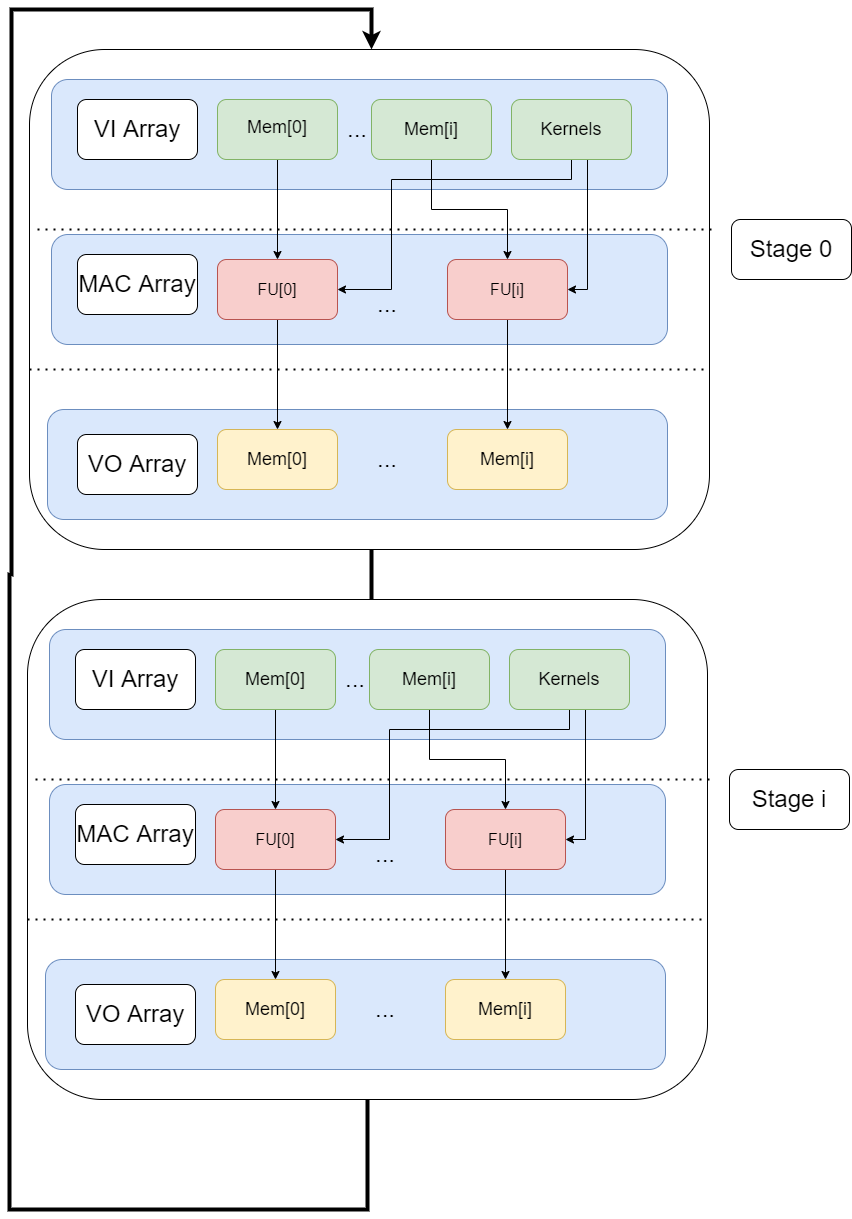
\includegraphics[width=0.7\textwidth]{Figures/Convolution.drawio.png}
    \caption{Versat Configuration goal in Graphical form}
    \label{VersatConfiguration}
\end{figure}

\subsection{Loading Data}

Usually, when doing a convolution in CPU, the frameworks transform the convolution to a matrix multiplication by creating a new matrix that will multiply with a
kernel vector. It's done this way as matrix multiply is a heavily optimized operation and can take advantage of a CPU's SIMD units or even call the GPU APIs
and offset the workload there. On Versat, this is not needed as to calculate one output, we will need only enough space in mem to hold
k\textsuperscript{2}*ch where ch is the channels of the input. And as such, it means 9216 bytes per VI at least for YoloV3 CNN when using 16-bit operands.

To load the data onto the mems in Versat, we will load segmented data. That is, for each mem, we will load the data
needed to do y iterations or y\textsubscript{3} iterations, depending on which convolution scenario it is.
The more inputs are transferred to a VI mem, the more efficient it is as data doesn't need to be replicated as much between the instances,
i.e. for the first output, there's a need for k\textsuperscript{2}*ch inputs, but for other sequential outputs, if the stride is one only k*ch more inputs are needed.
of course, this is only true if the stride is lower than the kernel size.

On the code, this takes form in one single line, thus the importance of the previously written functions.

\lstinputlisting[label=listing:memread,language=C++,frame=single,breaklines=true,firstline=446,lastline=446,caption=Load Input Matrix into VIs]{./Code/versat_configurations.cpp}

where the variable "size per channel" can be calculated with the following formula:

\[ size=w*(k+stride*(iter-1)) \]

where w is the width of the input matrix, k is the kernel size and iter is the number of iterations that this mem will run.

\subsection{Convolution Scenarios}
\label{ConvolutionScenarios}

When writing the configurations of the convolution runs, there are several cases the software needs to take into consideration.
As explained in the previous subsection, the data that the VIs can handle and the number of datapaths that the data can have influenced
the convolution scenarios. For this function, four were implemented and are presented in figure \ref{ConvScenarioss}.

\begin{figure}[!htbp]
    \centering
    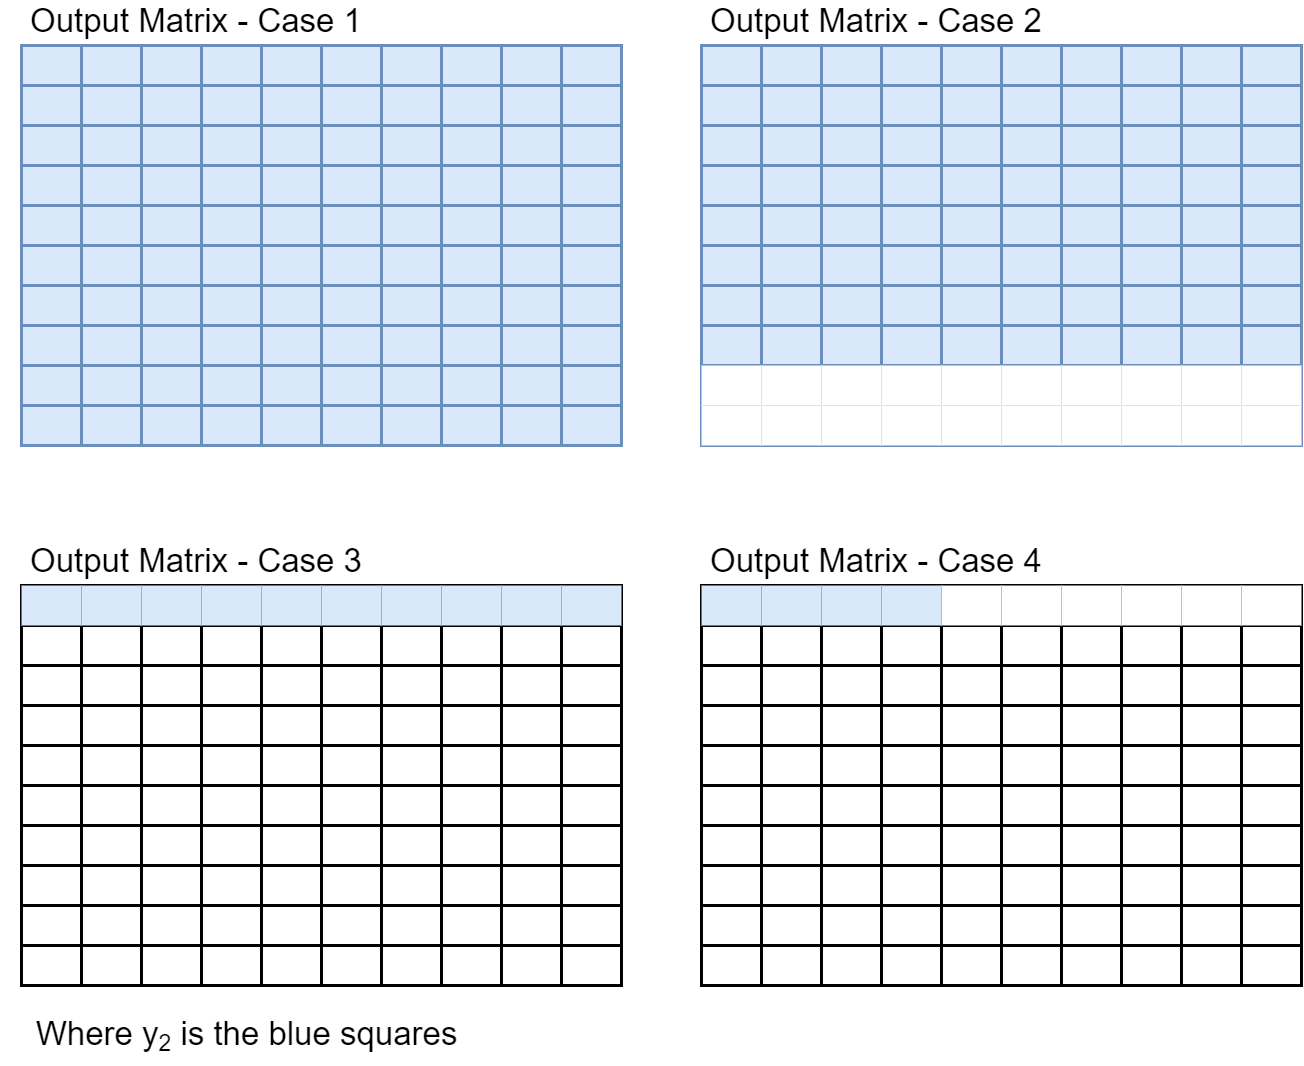
\includegraphics[width=0.7\textwidth]{Figures/Variables.drawio.png}
    \caption{Convolution Scenarios that Versat will have}
    \label{ConvScenarioss}
\end{figure}

The different hardware configurations and the endless possibilities for convolutions mean that all possibilities are covered. 
The only limitation of this generic function is to make partial results which is the last possible case where the mem can't handle enough inputs for 
1 output.

In figure \ref{ConvFlowChart}, the flowchart of each case is presented.

\newpage
\begin{figure}[!htbp]
    \centering
    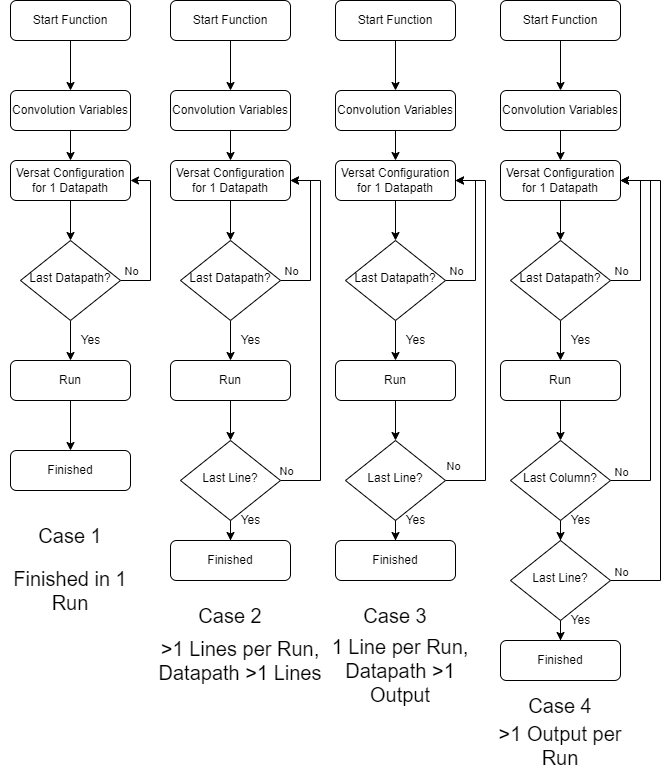
\includegraphics[width=0.65\textwidth]{Figures/ConvolutionFlowChart.drawio.png}
    \caption{Configuration Flowchart for the different scenarios}
    \label{ConvFlowChart}
\end{figure} 

And on listing \ref{listing:convfinal} the AGU configurations of the VIs that hold the input matrix, the MAC configuration, and finally
the VO AGU configuration.

\lstinputlisting[label=listing:convfinal,language=C++,frame=single,breaklines=true,firstline=449,lastline=478,caption=Versat configurations for one datapath]{./Code/versat_configurations.cpp}


